% Options for packages loaded elsewhere
\PassOptionsToPackage{unicode}{hyperref}
\PassOptionsToPackage{hyphens}{url}
%
\documentclass[
]{article}
\usepackage{amsmath,amssymb}
\usepackage{iftex}
\ifPDFTeX
  \usepackage[T1]{fontenc}
  \usepackage[utf8]{inputenc}
  \usepackage{textcomp} % provide euro and other symbols
\else % if luatex or xetex
  \usepackage{unicode-math} % this also loads fontspec
  \defaultfontfeatures{Scale=MatchLowercase}
  \defaultfontfeatures[\rmfamily]{Ligatures=TeX,Scale=1}
\fi
\usepackage{lmodern}
\ifPDFTeX\else
  % xetex/luatex font selection
\fi
% Use upquote if available, for straight quotes in verbatim environments
\IfFileExists{upquote.sty}{\usepackage{upquote}}{}
\IfFileExists{microtype.sty}{% use microtype if available
  \usepackage[]{microtype}
  \UseMicrotypeSet[protrusion]{basicmath} % disable protrusion for tt fonts
}{}
\makeatletter
\@ifundefined{KOMAClassName}{% if non-KOMA class
  \IfFileExists{parskip.sty}{%
    \usepackage{parskip}
  }{% else
    \setlength{\parindent}{0pt}
    \setlength{\parskip}{6pt plus 2pt minus 1pt}}
}{% if KOMA class
  \KOMAoptions{parskip=half}}
\makeatother
\usepackage{xcolor}
\usepackage[margin=1in]{geometry}
\usepackage{color}
\usepackage{fancyvrb}
\newcommand{\VerbBar}{|}
\newcommand{\VERB}{\Verb[commandchars=\\\{\}]}
\DefineVerbatimEnvironment{Highlighting}{Verbatim}{commandchars=\\\{\}}
% Add ',fontsize=\small' for more characters per line
\usepackage{framed}
\definecolor{shadecolor}{RGB}{248,248,248}
\newenvironment{Shaded}{\begin{snugshade}}{\end{snugshade}}
\newcommand{\AlertTok}[1]{\textcolor[rgb]{0.94,0.16,0.16}{#1}}
\newcommand{\AnnotationTok}[1]{\textcolor[rgb]{0.56,0.35,0.01}{\textbf{\textit{#1}}}}
\newcommand{\AttributeTok}[1]{\textcolor[rgb]{0.13,0.29,0.53}{#1}}
\newcommand{\BaseNTok}[1]{\textcolor[rgb]{0.00,0.00,0.81}{#1}}
\newcommand{\BuiltInTok}[1]{#1}
\newcommand{\CharTok}[1]{\textcolor[rgb]{0.31,0.60,0.02}{#1}}
\newcommand{\CommentTok}[1]{\textcolor[rgb]{0.56,0.35,0.01}{\textit{#1}}}
\newcommand{\CommentVarTok}[1]{\textcolor[rgb]{0.56,0.35,0.01}{\textbf{\textit{#1}}}}
\newcommand{\ConstantTok}[1]{\textcolor[rgb]{0.56,0.35,0.01}{#1}}
\newcommand{\ControlFlowTok}[1]{\textcolor[rgb]{0.13,0.29,0.53}{\textbf{#1}}}
\newcommand{\DataTypeTok}[1]{\textcolor[rgb]{0.13,0.29,0.53}{#1}}
\newcommand{\DecValTok}[1]{\textcolor[rgb]{0.00,0.00,0.81}{#1}}
\newcommand{\DocumentationTok}[1]{\textcolor[rgb]{0.56,0.35,0.01}{\textbf{\textit{#1}}}}
\newcommand{\ErrorTok}[1]{\textcolor[rgb]{0.64,0.00,0.00}{\textbf{#1}}}
\newcommand{\ExtensionTok}[1]{#1}
\newcommand{\FloatTok}[1]{\textcolor[rgb]{0.00,0.00,0.81}{#1}}
\newcommand{\FunctionTok}[1]{\textcolor[rgb]{0.13,0.29,0.53}{\textbf{#1}}}
\newcommand{\ImportTok}[1]{#1}
\newcommand{\InformationTok}[1]{\textcolor[rgb]{0.56,0.35,0.01}{\textbf{\textit{#1}}}}
\newcommand{\KeywordTok}[1]{\textcolor[rgb]{0.13,0.29,0.53}{\textbf{#1}}}
\newcommand{\NormalTok}[1]{#1}
\newcommand{\OperatorTok}[1]{\textcolor[rgb]{0.81,0.36,0.00}{\textbf{#1}}}
\newcommand{\OtherTok}[1]{\textcolor[rgb]{0.56,0.35,0.01}{#1}}
\newcommand{\PreprocessorTok}[1]{\textcolor[rgb]{0.56,0.35,0.01}{\textit{#1}}}
\newcommand{\RegionMarkerTok}[1]{#1}
\newcommand{\SpecialCharTok}[1]{\textcolor[rgb]{0.81,0.36,0.00}{\textbf{#1}}}
\newcommand{\SpecialStringTok}[1]{\textcolor[rgb]{0.31,0.60,0.02}{#1}}
\newcommand{\StringTok}[1]{\textcolor[rgb]{0.31,0.60,0.02}{#1}}
\newcommand{\VariableTok}[1]{\textcolor[rgb]{0.00,0.00,0.00}{#1}}
\newcommand{\VerbatimStringTok}[1]{\textcolor[rgb]{0.31,0.60,0.02}{#1}}
\newcommand{\WarningTok}[1]{\textcolor[rgb]{0.56,0.35,0.01}{\textbf{\textit{#1}}}}
\usepackage{graphicx}
\makeatletter
\def\maxwidth{\ifdim\Gin@nat@width>\linewidth\linewidth\else\Gin@nat@width\fi}
\def\maxheight{\ifdim\Gin@nat@height>\textheight\textheight\else\Gin@nat@height\fi}
\makeatother
% Scale images if necessary, so that they will not overflow the page
% margins by default, and it is still possible to overwrite the defaults
% using explicit options in \includegraphics[width, height, ...]{}
\setkeys{Gin}{width=\maxwidth,height=\maxheight,keepaspectratio}
% Set default figure placement to htbp
\makeatletter
\def\fps@figure{htbp}
\makeatother
\setlength{\emergencystretch}{3em} % prevent overfull lines
\providecommand{\tightlist}{%
  \setlength{\itemsep}{0pt}\setlength{\parskip}{0pt}}
\setcounter{secnumdepth}{-\maxdimen} % remove section numbering
\usepackage{mathpazo}
\usepackage{booktabs}
\usepackage{rotating}
\usepackage{makecell}
\usepackage{hyperref}
%% \usepackage[a4paper,margin=2cm]{geometry}


\newcommand{\orcidlogo}{\textcolor{orcidlogocol}{\aiOrcid}}
\usepackage[font=Large,labelfont=bf,textfont=bf]{caption}
\DeclareCaptionLabelFormat{addC}{#1 C#2}


%% This solution for adding the ORCID logo was taken from:
%% https://tex.stackexchange.com/questions/445563/ieeetran-how-to-include-orcid-in-tex-pdf-with-pdflatex/445583
%% and adapted simply by scaling the icon a little smaller than | to +
\usepackage{scalerel}
\usepackage{tikz}
\usetikzlibrary{svg.path}

\definecolor{orcidlogocol}{HTML}{A6CE39}
\tikzset{
  orcidlogo/.pic={
    \fill[orcidlogocol] svg{M256,128c0,70.7-57.3,128-128,128C57.3,256,0,198.7,0,128C0,57.3,57.3,0,128,0C198.7,0,256,57.3,256,128z};
    \fill[white] svg{M86.3,186.2H70.9V79.1h15.4v48.4V186.2z}
                 svg{M108.9,79.1h41.6c39.6,0,57,28.3,57,53.6c0,27.5-21.5,53.6-56.8,53.6h-41.8V79.1z M124.3,172.4h24.5c34.9,0,42.9-26.5,42.9-39.7c0-21.5-13.7-39.7-43.7-39.7h-23.7V172.4z}
                 svg{M88.7,56.8c0,5.5-4.5,10.1-10.1,10.1c-5.6,0-10.1-4.6-10.1-10.1c0-5.6,4.5-10.1,10.1-10.1C84.2,46.7,88.7,51.3,88.7,56.8z};
  }
}

\newcommand\orcidicon[1]{\href{https://orcid.org/#1}{\mbox{\scalerel*{

\begin{tikzpicture}[yscale=-1,transform shape]
\pic{orcidlogo};
\end{tikzpicture}
}{+}}}}

%% Set hyperlinks in colour to the "CODECHECK colour".
\hypersetup{colorlinks=true, urlcolor = [rgb]{0,.5,0.2}}
\ifLuaTeX
  \usepackage{selnolig}  % disable illegal ligatures
\fi
\usepackage{bookmark}
\IfFileExists{xurl.sty}{\usepackage{xurl}}{} % add URL line breaks if available
\urlstyle{same}
\hypersetup{
  pdftitle={CODECHECK certificate 2025-020},
  hidelinks,
  pdfcreator={LaTeX via pandoc}}

\title{CODECHECK certificate 2025-020}
\usepackage{etoolbox}
\makeatletter
\providecommand{\subtitle}[1]{% add subtitle to \maketitle
  \apptocmd{\@title}{\par {\large #1 \par}}{}{}
}
\makeatother
\subtitle{\url{https://doi.org/10.5281/zenodo.16758977}}
\author{}
\date{\vspace{-2.5em}}

\begin{document}
\maketitle

\centerline{\includegraphics[width=4cm]{C:/Users/langt/AppData/Local/R/win-library/4.3/codecheck/extdata/codecheck_logo.pdf}}\vspace*{2cm}

\begin{center}
\includegraphics[width=0.4\linewidth]{../img/Amsterdam_UMC_logo_with_text} \end{center}

\begin{table}[ht]
\centering
\begin{tabular}{lp{10cm}}
  \hline
Item & Value \\ 
  \hline
Title & AbSolution Report v.0.71
 \\ 
  Authors & Rodrigo García Valiente \orcidicon{0000-0003-0444-5587}  \\ 
  Reference & See 'report template' in Results folder \\ 
  Codechecker & Sam Langton \orcidicon{0000-0002-1322-1553}  \\ 
  Date of check & 2025-01-29 14:00:00 \\ 
  Summary & RMarkdown file with embedded R code created from the AbSolution Shiny app for the purposes of reproducibility.
 \\ 
  Repository & \url{https://github.com/langtonhugh/absolution_codecheck} \\ 
   \hline
\end{tabular}
\caption{CODECHECK summary} 
\end{table}

\begin{table}[ht]
\centering
\begin{tabular}{p{6cm}p{6cm}p{2cm}}
  \hline
Output & Comment & Size (b) \\ 
  \hline
\href{https://github.com/langtonhugh/absolution_codecheck/blob/master/codecheck/outputs/table1.png}{\path{screenshots/table1.png}} & Screenshot Table 1 & 9749 \\ 
  \href{https://github.com/langtonhugh/absolution_codecheck/blob/master/codecheck/outputs/figure1.png}{\path{screenshots/figure1.png}} & Screenshot Figure 1 & 19642 \\ 
  \href{https://github.com/langtonhugh/absolution_codecheck/blob/master/codecheck/outputs/figure2.png}{\path{screenshots/figure2.png}} & Screenshot Figure 2 & 11448 \\ 
  \href{https://github.com/langtonhugh/absolution_codecheck/blob/master/codecheck/outputs/figure3.png}{\path{screenshots/figure3.png}} & Screenshot Figure 3 & 33635 \\ 
  \href{https://github.com/langtonhugh/absolution_codecheck/blob/master/codecheck/outputs/figure4.png}{\path{screenshots/figure4.png}} & Screenshot Figure 4 & 27092 \\ 
   \hline
\end{tabular}
\caption{Summary of output files generated} 
\end{table}

\section{Summary}\label{summary}

This code was straightforward to codecheck. As per the ENCORE\footnote{\url{https://github.com/EDS-Bioinformatics-Laboratory/ENCORE}}
structure, there was a \texttt{renv} lockfile located in the
\texttt{0\_SoftwareEnvironment} folder. I created an \texttt{.RProj}
file in the root directory and copied over the lock file so that upon
executing \texttt{renv::restore()} it would be easily recognised. I
updated my R version to match the lockfile too. The AbSolution package
itself was installed from the pre-existing
\texttt{0\_SoftwareEnvironment} folder using
\texttt{install.packages("0\_SoftwareEnvironment/R/AbSolution\_0.0.5.9550.tar",\ repos\ =\ NULL,\ type="source")}.

I could then knit the RMarkdown file and it executed with no errors
first time. The tables and figures are printed directly in the HTML
output. The figures are interactive. For the purposes of this codecheck,
I made a screenshot of each one. The resulting HTML output file matches
the given file as expected. I did not test the docker file as the
outputs were reproduced on a Windows machine using \texttt{renv}, so
there was no need to delve into this for a codecheck.

\clearpage

\subsection{Recommendations}\label{recommendations}

The project was straightforward to reproduce so there are no specific
recommendations for improvement. I'd be interested to know how the
authors predict users will make use of the \texttt{renv} lock file in
the absence of any instructions. The lock file in the pre-existing
software environment folder is a \texttt{.prod} file extension (i.e.,
not \texttt{.lock}, which is the default for \texttt{renv}). For me,
\texttt{renv} did not recognise the lock file until I changed the file
extension to \texttt{.lock} and placed it in the root folder.

\clearpage

\section{Manifest files}\label{manifest-files}

\subsection{table1.png}\label{table1.png}

\textbf{Comment:} Screenshot Table 1

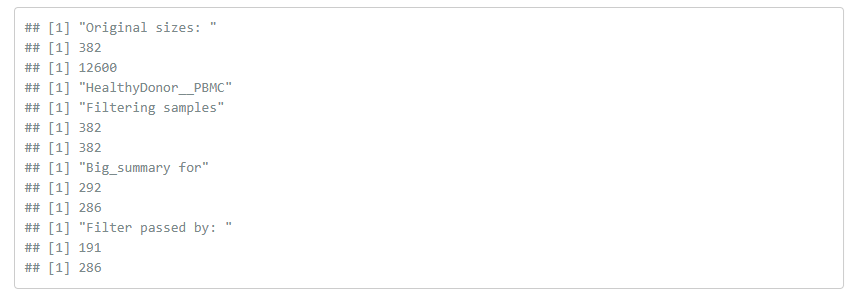
\includegraphics{C:/Users/langt/Documents/GitHub/absolution_codecheck/codecheck/outputs/table1.png}
\clearpage 

\subsection{figure1.png}\label{figure1.png}

\textbf{Comment:} Screenshot Figure 1

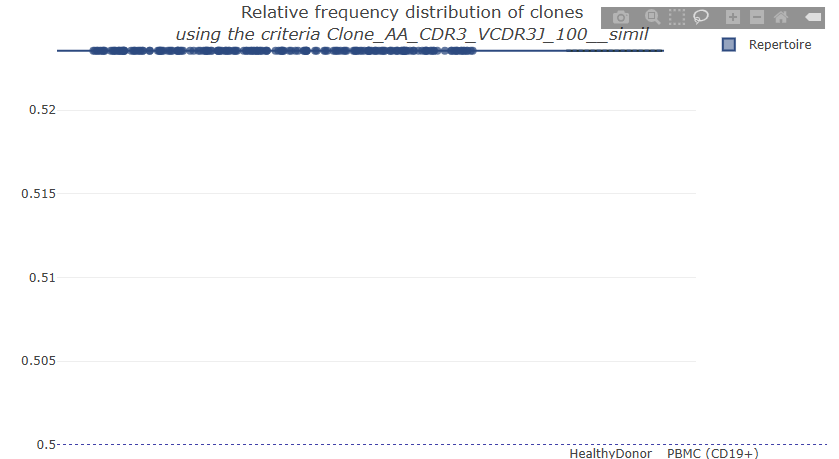
\includegraphics{C:/Users/langt/Documents/GitHub/absolution_codecheck/codecheck/outputs/figure1.png}
\clearpage 

\subsection{figure2.png}\label{figure2.png}

\textbf{Comment:} Screenshot Figure 2

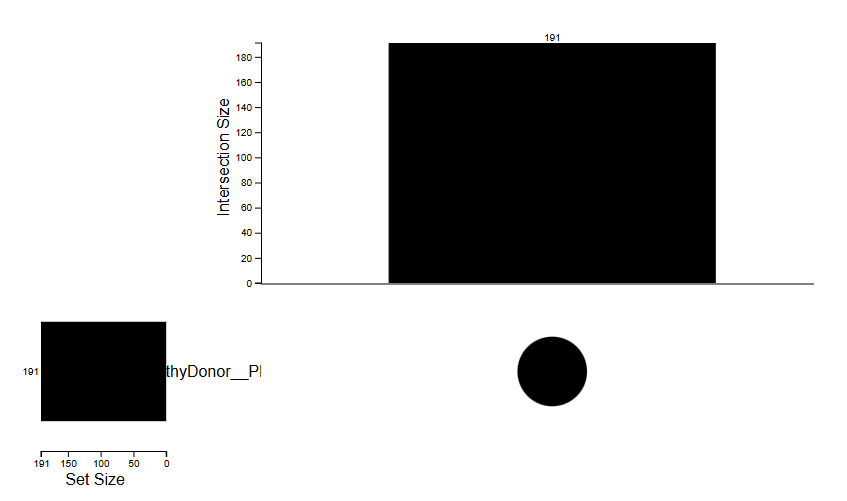
\includegraphics{C:/Users/langt/Documents/GitHub/absolution_codecheck/codecheck/outputs/figure2.png}
\clearpage 

\subsection{figure3.png}\label{figure3.png}

\textbf{Comment:} Screenshot Figure 3

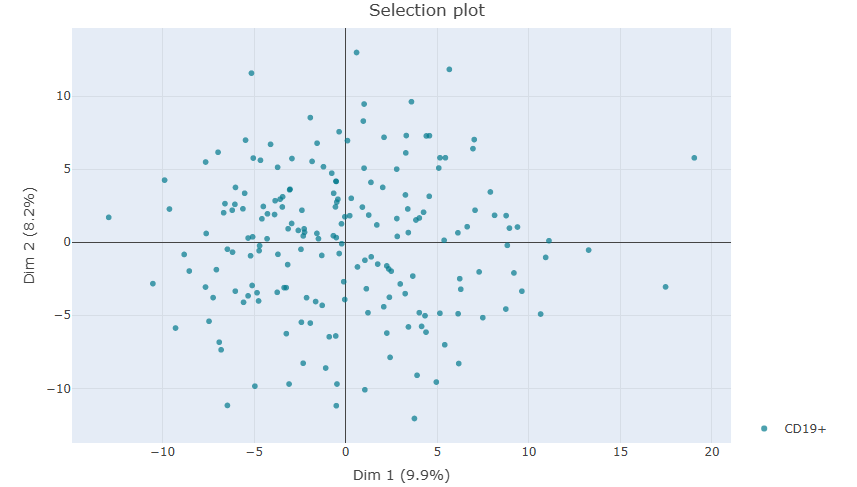
\includegraphics{C:/Users/langt/Documents/GitHub/absolution_codecheck/codecheck/outputs/figure3.png}
\clearpage 

\subsection{figure4.png}\label{figure4.png}

\textbf{Comment:} Screenshot Figure 4

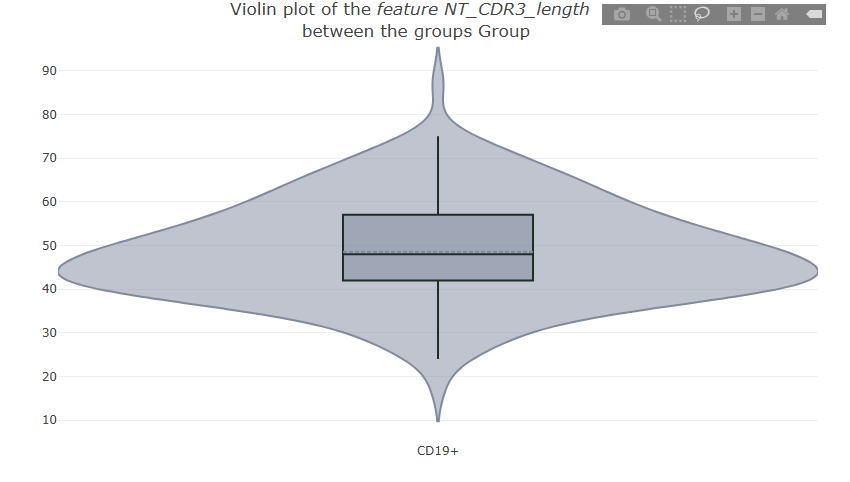
\includegraphics{C:/Users/langt/Documents/GitHub/absolution_codecheck/codecheck/outputs/figure4.png}
\clearpage 

\clearpage

\section{Citing this document}\label{citing-this-document}

Sam Langton (2025). CODECHECK Certificate 2025-XYZ. Zenodo.
\url{https://doi.org/10.5281/zenodo.FIXME}

\section{About CODECHECK}\label{about-codecheck}

This certificate confirms that the codechecker could independently
reproduce the results of a computational analysis given the data and
code from a third party. A CODECHECK does not check whether the original
computation analysis is correct. However, as all materials required for
the reproduction are freely available by following the links in this
document, the reader can then study for themselves the code and data.

\section{Session info}\label{session-info}

The following session info was saved after successful completion of the
codecheck.

\begin{Shaded}
\begin{Highlighting}[]
\FunctionTok{read.delim}\NormalTok{(}\StringTok{"sessionInfo.txt"}\NormalTok{)}
\end{Highlighting}
\end{Shaded}

\begin{verbatim}
##                                            R.version.4.3.1..2023.06.16.ucrt.
## 1                                  Platform: x86_64-w64-mingw32/x64 (64-bit)
## 2                                Running under: Windows 11 x64 (build 22621)
## 3                                                   Matrix products: default
## 4                                                                    locale:
## 5                                 [1] LC_COLLATE=English_United States.utf8 
## 6                                 [2] LC_CTYPE=English_United States.utf8   
## 7                                 [3] LC_MONETARY=English_United States.utf8
## 8                                 [4] LC_NUMERIC=C                          
## 9                                 [5] LC_TIME=English_United States.utf8    
## 10                                               time zone: Europe/Amsterdam
## 11                                                   tzcode source: internal
## 12                                                   attached base packages:
## 13 [1] stats     graphics  grDevices utils     datasets  methods   base     
## 14                                                  other attached packages:
## 15     [1] plotly_4.10.1         ggplot2_3.5.1         dplyr_1.1.2          
## 16                           [4] shiny_1.7.4           AbSolution_0.0.5.9550
## 17                                loaded via a namespace (and not attached):
## 18               [1] shinythemes_1.2.0           later_1.3.1                
## 19               [3] bitops_1.0-7                tibble_3.2.1               
## 20               [5] Peptides_2.4.5              R.oo_1.25.0                
## 21               [7] shinymanager_1.0.410        lifecycle_1.0.3            
## 22               [9] shinyjqui_0.4.1             doParallel_1.0.17          
## 23              [11] rprojroot_2.0.3             lattice_0.20-45            
## 24              [13] MASS_7.3-58.2               crosstalk_1.2.0            
## 25              [15] magrittr_2.0.3              sass_0.4.6                 
## 26              [17] rmarkdown_2.21              jquerylib_0.1.4            
## 27              [19] yaml_2.3.7                  bigparallelr_0.3.2         
## 28              [21] httpuv_1.6.11               askpass_1.1                
## 29              [23] reticulate_1.34.0           cowplot_1.1.1              
## 30              [25] DBI_1.2.3                   RColorBrewer_1.1-3         
## 31              [27] ade4_1.7-22                 golem_0.4.1                
## 32              [29] zlibbioc_1.46.0             R.cache_0.16.0             
## 33              [31] GenomicRanges_1.52.0        purrr_1.0.1                
## 34              [33] R.utils_2.12.2              BiocGenerics_0.46.0        
## 35              [35] RCurl_1.98-1.12             styler_1.10.0              
## 36              [37] bigassertr_0.1.6            reactable_0.4.4            
## 37              [39] GenomeInfoDbData_1.2.10     IRanges_2.34.0             
## 38              [41] S4Vectors_0.38.1            umap_0.2.10.0              
## 39              [43] RSpectra_0.16-1             parallelly_1.35.0          
## 40              [45] codetools_0.2-19            DelayedArray_0.26.7        
## 41              [47] DT_0.28                     bs4Dash_2.3.4              
## 42              [49] tidyselect_1.2.0            bigstatsr_1.5.12           
## 43              [51] viridis_0.6.3               shinyWidgets_0.7.6         
## 44              [53] matrixStats_1.2.0           stats4_4.3.1               
## 45              [55] flock_0.7                   GenomicAlignments_1.36.0   
## 46              [57] jsonlite_1.8.4              ellipsis_0.3.2             
## 47              [59] dashboardthemes_1.1.6       iterators_1.0.14           
## 48              [61] foreach_1.5.2               tools_4.3.1                
## 49              [63] progress_1.2.2              stringdist_0.9.10          
## 50              [65] Rcpp_1.0.10                 glue_1.6.2                 
## 51              [67] gridExtra_2.3               xfun_0.46                  
## 52              [69] MatrixGenerics_1.12.3       GenomeInfoDb_1.36.0        
## 53              [71] withr_2.5.0                 formatR_1.14               
## 54              [73] fastmap_1.1.1               sourcetools_0.1.7-1        
## 55              [75] fansi_1.0.4                 shinyjs_2.1.0              
## 56              [77] openssl_2.0.6               digest_0.6.31              
## 57              [79] R6_2.5.1                    mime_0.12                  
## 58              [81] colorspace_2.1-0            RSQLite_2.3.1              
## 59              [83] diptest_0.76-0              R.methodsS3_1.8.2          
## 60              [85] config_0.3.2                utf8_1.2.3                 
## 61              [87] tidyr_1.3.0                 generics_0.1.3             
## 62              [89] data.table_1.16.2           iterors_1.0                
## 63              [91] prettyunits_1.1.1           httr_1.4.6                 
## 64              [93] htmlwidgets_1.6.2           S4Arrays_1.0.4             
## 65              [95] pkgconfig_2.0.3             gtable_0.3.3               
## 66              [97] blob_1.2.4                  shinymeta_0.2.0.3          
## 67              [99] XVector_0.40.0              htmltools_0.5.5            
## 68             [101] scales_1.3.0                fresh_0.2.0                
## 69             [103] Biobase_2.60.0              sunburstR_2.1.8            
## 70             [105] png_0.1-8                   attempt_0.3.1              
## 71             [107] knitr_1.42                  rstudioapi_0.14            
## 72             [109] tzdb_0.4.0                  nlme_3.1-162               
## 73             [111] cachem_1.0.8                stringr_1.5.0              
## 74             [113] KernSmooth_2.23-20          parallel_4.3.1             
## 75             [115] shinycssloaders_1.0.0       pillar_1.9.0               
## 76             [117] grid_4.3.1                  vctrs_0.6.5                
## 77             [119] shazam_1.2.0                promises_1.2.0.1           
## 78             [121] shinyFiles_0.9.3            airr_1.4.1                 
## 79             [123] xtable_1.8-4                billboarder_0.4.0          
## 80             [125] evaluate_0.21               readr_2.1.4                
## 81             [127] cli_3.6.1                   compiler_4.3.1             
## 82             [129] Rsamtools_2.16.0            rlang_1.1.1                
## 83             [131] crayon_1.5.2                sortable_0.5.0             
## 84             [133] fs_1.6.2                    stringi_1.7.12             
## 85             [135] viridisLite_0.4.2           BiocParallel_1.34.1        
## 86             [137] assertthat_0.2.1            munsell_0.5.0              
## 87             [139] Biostrings_2.68.1           lazyeval_0.2.2             
## 88             [141] upsetjs_1.11.1              Matrix_1.6-5               
## 89             [143] benchmarkme_1.0.8           scrypt_0.1.6               
## 90             [145] hms_1.1.3                   alakazam_1.3.0             
## 91             [147] bit64_4.0.5                 learnr_0.11.5              
## 92             [149] seqinr_4.2-30               SummarizedExperiment_1.30.1
## 93             [151] igraph_1.6.0                memoise_2.0.1              
## 94             [153] bslib_0.4.2                 benchmarkmeData_1.0.4      
## 95             [155] bit_4.0.5                   ape_5.7-1
\end{verbatim}

\end{document}
